\documentclass[11pt]{article}
\usepackage[margin=1in]{geometry}
\usepackage{amssymb,amsfonts,amsmath,amsthm,amscd,dsfont,mathrsfs,bbold}
\usepackage{blkarray}
\usepackage{graphicx,float,psfrag,epsfig,color}
\usepackage{microtype}
\usepackage[pdftex,pagebackref=true,colorlinks]{hyperref}
\usepackage{tikz}
\usetikzlibrary{positioning}
\tikzset{main node/.style={circle,fill=white!20,draw,minimum size=1cm,inner sep=0pt},}
\hypersetup{linkcolor=[rgb]{.7,0,0}}
\hypersetup{citecolor=[rgb]{0,.7,0}}
\hypersetup{urlcolor=[rgb]{.7,0,.7}}

\newcommand{\remove}[1]{}
\setlength{\topmargin}{0.2in} \setlength{\headheight}{0in}
\setlength{\headsep}{0in} \setlength{\textheight}{8.7in}
\setlength{\topsep}{0in} \setlength{\itemsep}{0in}
\parskip=0.060in

\textwidth=6.6in \oddsidemargin=0truecm \evensidemargin=0truecm



\hbadness=10000 \vbadness=10000

\setlength{\oddsidemargin}{.25in}
\setlength{\evensidemargin}{.25in} \setlength{\textwidth}{6in}
\setlength{\topmargin}{-0.4in} \setlength{\textheight}{8.5in}

\newcommand{\details}[8]{
	\renewcommand{\thepage}{#1-\arabic{page}}
	\noindent
	\begin{center}
		\framebox{
			\vbox{
				\hbox to 5.78in { {\bf  Advanced Methods in Machine Learning}\hfill #2}
				\vspace{4mm}
				\hbox to 5.78in { {\Large \hfill Exercise #1  \hfill} }
				\vspace{2mm}
				\hbox to 5.78in { {{\it #3} \hfil {\it #4} \hfil {\it #5}} }
				\vspace{2mm}
				\hbox to 5.78in { {{\it #6} \hfil {\it #7} \hfil {\it #8}} }
			}
		}
	\end{center}
	\vspace*{4mm}
}

\newcommand{\lecture}[8]{\details{#1}{#2}{#3}{#4}{#5}{#6}{#7}{#8}}





\begin{document}
	\lecture{1}{25.3.2018}{Nir Raviv 200683548}{Roi Tabach 203022983}{Andrey Leshenko 322026527}{nirraviv@mail.tau.ac.il}{roi.tabach@gmail.com}{andrey.leshenko@gmail.com}
	
	\part*{Q1}
	Given a distribution $q$ over three random variables $X_1, X_2, X_3$:
\begin{equation}
q(x_1, x_2, x_3) = \begin{cases}
1/12, & x_1 \oplus x_2 \oplus x_3 = 0\\
1/6, & x_1 \oplus x_2 \oplus x_3 = 1\\
\end{cases}
\end{equation}
\section*{a}
First, we will find $I(q)$, the set of all conditional independence statements.
Because of the commutativity of the XOR operation, there is no difference between the variables.
We will look at the probability tables of two variables depending on the value of the third:
\begin{center}

\begin{tabular}{| c | c | c |}
\hline
$\boldsymbol{x_3=0}$ & $\boldsymbol{x_3=1}$ & $\boldsymbol{x_3=*}$ \\
\hline\hline
\begin{tabular}{ c|c c } 
  & $x_2=0$ & $x_2=1$ \\ 
 \hline
 $x_1=0$ & $1/12$ & $1/6$ \\ 
 $x_1=1$ & $1/6$ & $1/12$ \\ 
\end{tabular}
&
\begin{tabular}{ c|c c } 
  & $x_2=0$ & $x_2=1$ \\ 
 \hline
 $x_1=0$ & $1/6$ & $1/12$ \\ 
 $x_1=1$ & $1/12$ & $1/6$ \\ 
\end{tabular}
&
\begin{tabular}{ c|c c } 
  & $x_2=0$ & $x_2=1$ \\ 
 \hline
 $x_1=0$ & $3/12$ & $3/12$ \\ 
 $x_1=1$ & $3/12$ & $3/12$ \\ 
\end{tabular}
\\
\hline
\end{tabular}
\end{center}
We can see that two variables ($x_1,x_2$ in this case) are dependent when given the value of the third variable ($x_3$),
but are \textit{independent} when this value is unknown.
This means that the set of conditional independences contains exactly all pairs of variables:
\begin{equation}
I(q) = \{X_1 \bot X_2, X_1 \bot X_3, X_2 \bot X_3\}
\end{equation}

\section*{b}
We will show that there is no DAG $G$ where $I_{LM}(G)=I(q)$.
The Local Markov properties are defined as:

\begin{equation}
X_i \bot X_{ND(i) \setminus Pa(i)} | X_{Pa(i)}\qquad i=1,\ldots,n
\end{equation}

If we want to have $(X_1 \bot X_2) \in I_{LM}(G)$ then $X_2$ must not be a descendant of $X_1$,
and it can't be its parent.
Taking the other CI-s into account, no variable can be a parent of any other variable.
The only possible graph is the graph where all variables are independent and there are no edges,
but in such case $I_{LM}$ will also contain $X_1 \bot X_2 | X_3$, which is not in $I(q)$.
Therefore there is no DAG $G$ where $I_{LM}(G)=I(q)$.

\section*{c}
We will show that there is no undirected graph $G$ such that $I_{sep}(G) = I(q)$.
The separation CI properties of a graph $G$ are defined as:

\begin{equation}
I_{sep}(G) = \{W \bot Y | Z : \text{$Z$ separates $W$ and $Y$ in $G$}\}
\end{equation}

If we want to have $(X_1 \bot X_2) \in I_{sep}(G)$ then $X_1$ and  $X_2$ must be somehow separated in the graph.
They can't be separated by $X_3$ because in such case $I_{sep}$ will also contain $X_1 \bot X_2 | X_3$, therefore they must be in different connected components.
Taking all of $I(q)$ into account, the only possible graph is the graph where all variables are independent and there are no edges.
But even in such case, because all variables are independent $I_{sep}$ will still contain $X_1 \bot X_2 | X_3$. Therefore there is no $G$ where $I_{sep}(G)=I(q)$.

	\part*{Q2}
	Given four random Variables: $X$, $Y$, $Z$, $W$, and a probability $p$ s.t. $p(x,y,z,w)>0$, and given
\begin{equation}\label{eq:q2given}
\left(X \perp Y \mid Z, W\right), \left(X \perp W \mid Z, Y\right)
\end{equation}
We need to show that 
\begin{equation}
\left(X \perp Y,W \mid Z\right)
\end{equation}
From \eqref{eq:q2given} we get $Pr(X|Y, Z, W) = Pr(X | Z, W)$ and also
\begin{equation}\label{eq:q2ontheway}
Pr(X|Y,Z,W)=Pr(X|Z,Y)
\end{equation}
So 
\begin{equation}\label{eq:q2conclusion}
Pr(X|Y,Z)=Pr(X|W,Z)
\end{equation}
And we will show that $Pr(X|Z)\cdot Pr(Y,W|Z)=Pr(X,Y,W|Z)$.
\begin{equation*}
Pr(X|Z)\cdot Pr(Y,W|Z) \overset{(a)}{=} \frac{Pr(X,Z)\cdot Pr(Y,W,Z)}{Pr^2(Z)}
\end{equation*}
(a) is due to the definition of conditional probability. This is equal, due to the law of total probability, to
\begin{equation*}
= \frac{\left[\sum_{w}Pr(W=w,X,Z)\right] \cdot Pr(Y,W,Z)}{Pr^2(Z)}
\overset{(b)}{=} \frac{\left[\sum_{w}Pr(Z, W=w)\cdot Pr(X|Z, W=w)\right] \cdot Pr(Y,W,Z)}{Pr^2(Z)}
\end{equation*}
(b) a characteristic of conditional probability. Now we can use \eqref{eq:q2conclusion}, replace $Pr(X|Z, W=w)$ with $Pr(X|Z, Y)$ and take it out of the sum (it's not dependent on $w$)
\begin{equation*}
= \frac{\left[\sum_{w}Pr(Z, W=w)\right]\cdot Pr(X|Z, Y) \cdot Pr(Y,W,Z)}{Pr^2(Z)} \overset{(c)}{=} \frac{Pr(X|Z, Y) \cdot Pr(Y,W,Z)}{Pr(Z)} 
\end{equation*}
(c) is again due to total probability, we were only left with $Pr(z)$ and it's simplified with the $1/Pr^2(Z)$ leaving $1/Pr(Z)$.
Now we use \eqref{eq:q2ontheway} with what is left, to get 
\begin{equation*}
= \frac{Pr(X|Z, W, Y) \cdot Pr(Y,W,Z)}{Pr(Z)} = \frac{Pr(X,Y,Z,W)}{Pr(Z)} = Pr(X,Y,W|Z)
\end{equation*}
$QED$

	\part*{Q3}
	$X_1,...,X_n$ are random variables.
	We must find the Markov blanket of $X_i$, the minimal subset $S$ s.t
	\begin{equation}\label{eq:q3given}
	\left( X_i \perp X_{\bar{S}\backslash i} \mid X_S \right)
	\end{equation}
	According to  \eqref{eq:q3given} we can find the subset $S$ by the following equation, 
	\begin{equation}
	\left. P(X_i|X_{\bar{S}\backslash i}, X_S) = P(X_i|X_S) \right.
	\end{equation}
	\begin{equation*}
	P(X_i|X_{\bar{S}\backslash i}, X_S) = P(X_i | X_1,...,X_{i-1},X_{i+1},...,X_n) = \frac{P(X_1,...,X_n)}{P(X_1,...,X_{i-1},X_{i+1},...,X_n)}
	\end{equation*}
	\begin{equation*}
	\overset{(a)}{=} \frac{\prod_{j=1}^n P(X_j|X_{Pa(j)})}{\sum_{X_i} P(X_1,...,X_n)} = \frac{\prod_{j=1}^n P(X_j|X_{Pa(j)})}{\sum_{X_i} \prod_{j=1}^n P(X_j|X_{Pa(j)})}
	\end{equation*}
	(a) is due to the property  of Bayesian network over a DAG G. \\*
	After cancellation of the common terms we remain with terms containing only $X_i$ as a child or a parent, \\*
	\begin{equation*}
		P(X_i|X_{\bar{S}\backslash i}, X_S) = \frac{P(X_i|X_{Pa(i)})\prod_{X_j\in X_{Ch(i)}} P(X_j|X_{Pa(j)})}{\sum_{X_i}P(X_i|X_{Pa(i)})\prod_{X_j\in X_{Ch(i)}} P(X_j|X_{Pa(j)})} = P(X_i|X_S)
	\end{equation*}
	Thus, $S = Pa(i) \cup Ch(i) \cup \bigcup_{X_j\in Ch(i)} Pa(j)$
\part*{Q4}
\section*{a}
We consider the graph described in the question.
We have seen in the slides that for positive distributions:
\begin{equation}\label{eq:q4a}
I(p)\supseteq I_{pair}(G) \rightarrow I(p)\supseteq I_{sep}(G)
\end{equation}

Since we are given a positive distribution $p$, it is suffice to show that:
$I(p)\supseteq I_{pair}(G)$.

And indeed, the very definition of $G=(V,E)$ given $p$ will give us the desired effect.
$I_{pair}(G)$ means that for every $(i,j)\notin E$,$X_i\perp X_j | X_{\{1\dots n\}\setminus\{i,j\}}$.
$E$ was defined so that if $\left(X_i\perp X_j | X_{\{1\dots n\}\setminus\{i,j\}}\right)$, then $(i,j)\notin E$.

We got $I(p) \supseteq I_{pair}(G)$. With \eqref{eq:q4a} we get $QED$.

\section*{b}
Now to show that removing a single edge from $G$ will result in it not being an I-map any more. Assuming we removed $(i,j)$ from $E$, we will show that there is an element in $I_{sep}(G')$ ($G'$ is the new $G$) which is not an element of $I(p)$. From the fact that $(i,j)$ was an edge, we can learn that
\begin{equation}\label{eq:q4b}
\left(X_i\perp X_j | X_{\{1\dots n\}\setminus\{i,j\}}\right)\notin I(p)
\end{equation}
Now we notice that the LHS in \eqref{eq:q4b} is an element of $I_{sep}(G')$, since indeed every path between $i$ and $j$ passes through the set of all the other nodes (if there isn't a path, so the claim is correct. If there is a path, it doesn't pass through the edge we removed, so there is a node in the path which is in the set $\{1\dots n\}\setminus\{i,j\}$).
Therefore $I_{sep}(G') \not\subseteq I(p)$, and $G'$ is not an I-map for $p$. $QED$. 
\part*{Q5}
A distribution $p(x_1,x_2,x_3,x_4)$ which has 1/8 probability for each of the assignments $(0,0,0,0),(1,0,0,0),(1,1,0,0),(1,1,1,0),(0,0,0,1),(0,0,1,1),(0,1,1,1),(1,1,1,1)$ and probability zero for all 	others is given. We need to show that $I_{sep}(G)\subseteq I(p)$ where G is a square graph but that $p$ is not a Markov network with respect to this graph. \\*
First, will show that $I_{sep}(G) \subseteq I(p)$ on the graph below: \\*
\begin{tikzpicture}
\begin{scope}[xshift=2cm]
\node[main node] (1) {$1$};
\node[main node] (2) [right = 1cm  of 1]  {$2$};
\node[main node] (3) [below = 1cm  of 2]  {$3$};
\node[main node] (4) [below = 1cm  of 1]  {$4$};

\path[draw,thick]
(1) edge node {} (2)
(2) edge node {} (3)
(3) edge node {} (4)
(4) edge node {} (1)
;
\end{scope}
\end{tikzpicture} \\*
To do this, we need to show the following conditions:
\begin{itemize}
	\item $X_1 \perp X_3 \mid (X_2, X_4)$
	\item $X_2 \perp X_4 \mid (X_1, X_3)$
\end{itemize}
By proving that $\Pr(x_1,x_2,x_3,x_4) = \Pr(x_4,x_3,x_2,x_1)$, proving the first condition is enough.
$\Pr(0,0,0,1) = \Pr(1,0,0,0) = \frac{1}{8}$, \\*
$\Pr(0,0,1,1) = \Pr(1,1,0,0) = \frac{1}{8}$, \\*
$\Pr(0,1,1,1) = \Pr(1,1,1,0) = \frac{1}{8}$, \\*
$\Pr(0,0,0,0) = \frac{1}{8}$, $\Pr(1,1,1,1) = \frac{1}{8}$ and the rest are zeros. \\*
To prove the first condition we need to show that whatever pair of values you choose from $(X_2,X_4)$, we can know either $X_1$ or $X_3$ with certainty, then conditioning on the other one provides 	no additional information.
\begin{itemize}
	\item If $(X_2,X_4) = (0,0)$ then $X_3=0$.
	\item If $(X_2,X_4) = (0,1)$ then $X_1=0$.
	\item If $(X_2,X_4) = (1,0)$ then $X_1=1$.
	\item If $(X_2,X_4) = (1,1)$ then $X_3=1$.
\end{itemize}
Finally, we need to show that $p$ is not a Markov network w.r.t G by contradiction of Hammersley-Clifford Theorem. Using pairwise MRF we can write the following: \\*
$\Pr(x_1,x_2,x_3,x_4) \propto \phi_{12}(x_1,x_2)\phi_{23}(x_2,x_3)\phi_{34}(x_3,x_4)\phi_{41}(x_4,x_1)$ \\*
The following equations are true:
\begin{description}
	\item[] $\phi_{12}(0,0)\phi_{23}(0,1)\phi_{34}(1,0)\phi_{41}(0,0) \propto p(0,0,1,0) = 0$
	\item[] $\phi_{12}(0,0)\phi_{23}(0,0)\phi_{34}(0,0)\phi_{41}(0,0) \propto p(0,0,0,0) = \frac{1}{8}$
	\item[] $\phi_{12}(0,0)\phi_{23}(0,1)\phi_{34}(1,1)\phi_{41}(1,0) \propto p(0,0,1,1) = \frac{1}{8}$
\end{description}
Then, if follows that $\phi_{34}(1,0)$ must be 0 which is a contradiction to the following: \\*
$\phi_{12}(1,1)\phi_{23}(1,1)\phi_{34}(1,0)\phi_{41}(0,1) \propto p(1,1,1,0) = \frac{1}{8}$. Thus, $p$ isn't Markov network on G.

\part*{Q6}
Let $G$ be a tree graph with edges $E$, and let $p(x)$ be a Markov network on this graph.
We will show that for any assignment $x_1,\ldots,x_n$ it holds:
\begin{equation}
p(x_1,\ldots,x_n) = \prod_{i=1}^{n}p(x_i) \prod_{ij\in E}\frac{p(x_i,x_j)}{p(x_i)p(x_j)}
\end{equation}

The proof is by induction, and uses the $I_{sep}$ conditional independence properties.
First will rename the nodes of the graph such that $x_1,\ldots,x_t$ is a connected sub-tree of $G$ for all $t$ (this can be done by for example taking the BFS traversal order of the tree).
The base cases are trivially seen by substituting into the equation:
\begin{align}
p(x_1) &= p(x_1) \\
p(x_1, x_2) &= p(x_1)p(x_2) \cdot \frac{p(x_1, x_2)}{p(x_1)p(x_2)} = p(x_1, x_2)
\end{align}
The induction hypothesis is that at step $t-1$, for $x_1,\ldots,x_{t-1}$ it holds that
\begin{equation}
p(x_1,\ldots,x_{t-1}) = \prod_{i=1}^{t-1}p(x_i) \prod_{ij\in E_{t-1}}\frac{p(x_i,x_j)}{p(x_i)p(x_j)}
\end{equation}
where $E_{t-1}$ are all edges which go between nodes of $x_1,\ldots,x_{t-1}$.
For the $t$-th step, from the way we ordered the nodes it is know that $E_t = E_{t-1}\cup\{jt\}$ for some $j < t$. To prove the induction hypothesis also holds for step $t$ we need to show that:
\begin{align}
p(x_1,\ldots,x_{t}) &\stackrel{?}{=} \left[ \prod_{i=1}^{t-1}p(x_i) \prod_{ij\in E_{t-1}}\frac{p(x_i,x_j)}{p(x_i)p(x_j)} \right] \cdot p(x_t)\frac{p(x_t,x_j)}{p(x_t)p(x_j)}\\
&\stackrel{?}{=} \left[p(x_1,\ldots,x_{t-1})\right] \cdot \frac{p(x_t,x_j)}{p(x_j)} \label{eq:q6step}
\end{align}

We know that node $t$ is connected to the rest of $x_1,\ldots,x_{t-1}$ through a single edge to some node $x_j$ where $j < i, jt\in E$.
The same edge we moved to the right of the previous equation!
The node $x_j$ separates $x_t$ from the rest of the nodes in $E_t$.
Therefore from the $I_{sep}(G)$ CI properties, we know that $X_t \bot (X_1,\ldots,X_{t-1}\setminus X_j) | X_j$. We will now use this property:

\begin{align}
p(x_1,\ldots,x_t) &= p(x_1,\ldots,x_{t-1})\cdot p(x_t | x_1,\ldots,x_{t-1}) \\
& = p(x_1,\ldots,x_{t-1})\cdot p(x_t | x_j)\\
& = p(x_1,\ldots,x_{t-1})\cdot \frac{p(x_t,x_j)}{p(x_j)}
\end{align}
This is just what we wanted to show at \eqref{eq:q6step}.
This proves the induction step and concludes the proof.

\end{document}
